\documentclass[tikz]{standalone}
\usepackage{pgfplots}
\pgfplotsset{width=7cm, compat=1.18}
\begin{document}
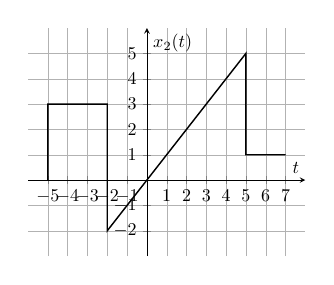
\begin{tikzpicture}[scale=0.65]
	\begin{axis}[
	axis y line=center,
	axis x line=middle,
	xmin=-6,	xmax=8,
	ymin=-3,	ymax=6,
	xlabel=$t$,
	ylabel=$x_2(t)$,
	xtick={-5,-4,-3,-2,-1,0,1,2,3,4,5,6,7},
	ytick={-2,-1,0,1,2,3,4,5},
	grid=both,
	grid style={line width=.1pt, draw=gray!40},
	major grid style={line width=.2pt,draw=gray!60},
	]
	\addplot[line width=.8pt] coordinates {(-5,0) (-5,3) (-2,3) (-2,-2) (5,5) (5,1) (7,1)};
\end{axis}
\end{tikzpicture}
\end{document}
